% TEMPLATE for Usenix papers, specifically to meet requirements of
%  USENIX '05
% originally a template for producing IEEE-format articles using LaTeX.
%   written by Matthew Ward, CS Department, Worcester Polytechnic Institute.
% adapted by David Beazley for his excellent SWIG paper in Proceedings,
%   Tcl 96
% turned into a smartass generic template by De Clarke, with thanks to
%   both the above pioneers
% use at your own risk.  Complaints to /dev/null.
% make it two column with no page numbering, default is 10 point

% Munged by Fred Douglis <douglis@research.att.com> 10/97 to separate
% the .sty file from the LaTeX source template, so that people can
% more easily include the .sty file into an existing document.  Also
% changed to more closely follow the style guidelines as represented
% by the Word sample file. 

% Note that since 2010, USENIX does not require endnotes. If you want
% foot of page notes, don't include the endnotes package in the 
% usepackage command, below.

\documentclass[letterpaper,twocolumn,10pt]{article}
\usepackage{usenix,epsfig,endnotes}
\begin{document}

%don't want date printed
\date{}

%make title bold and 14 pt font (Latex default is non-bold, 16 pt)
\title{\Large \bf Saving pins and power with integrated voltage converters}

\author{
{\rm Michael Barrow}\\
mbarrow@eng.ucsd.edu\\
University of California, San Diego
%\and
%{\rm Second Name}\\
%Second Institution
}

\maketitle

% Use the following at camera-ready time to suppress page numbers.
% Comment it out when you first submit the paper for review.
\thispagestyle{empty}


\subsection*{Abstract}
Recently, demand for increased processor performance coupled with reducing power budget has been addressed using emerging parallel processors. Parallel computation is an energy efficient \textbf{(cite chandrakasan)} way of increasing performance but requires wider interconnect busses. At the die boundary, the consequence is that systems face an IO bottleneck. The connection between silicon and substrate ends the scope of Moores law in a system, with IO density of packages increasing at a slower rate than on chip.\\
Compounding this problem, addressing performance by increasing paralell units result in increasing energy density due to the end of Dennard scaling \textbf{(cite)}. Devices therefore require an increasing number of power pins, further limiting IO pin availability. \textbf{HOW ABOUT COMPELLING EXAMPLE?}
We examine integrated power converters in this context. A review of the literature suggests with further research this technique could address the IO bottleneck of future processors.% and power efficiency of future processors.         

\section{Introduction}

%As Moores law continues, Technology scaling gives an increasing number of building blocks to meet conflicting consumer demands of increasing performance and energy efficiency. However the turn right approach exposes architects to complications of inconsistent technology scaling rates. In particular, for IO bound applications, the amount of achievable parallelism in silicon is proportional to the number of IO pins. The  \\

%\begin{itemize}
%\item{\textbf{Motivation}:  crisis has been known for some ti}
%\item{Stakeholders}
%\item{Historical context}
%\item{Current state of art}
%\item{State of art limitations}
%\item{Content of doc}
%\end{itemize}

Against a backdrop of declining PC and growing smartphone sales, mobile devices drive demand for low power, high performance architectures. Emerging applications such as augmented reality, location aware services, high performance games and novel machine interfaces place an increasing demand for expanded IO capabilities and memory bandwidth from generation to generation of these devices. With the number of popular software stacks being lower than the number of major hardware vendors, device battery life is an important product differentiator. Research interest has therefore increased in power efficient architectures that can meet the IO and memory bandwidth requirements of the mobile segment.\\
%DROP THISDespite a drop in PC demand, server 
\indent package IO density is a well known problem to architects. Marbell et al~\cite{Marbell2011} review 130 hardware designs over 30 years and conclude the historical trend of package pin count and power pin count increase at an unsustainable rate. Promising solutions have been proposed, with Chang et al~\cite{Chang2010} identifying a subset of practical approaches in 2010. They conclude that voltage scaling as proposed by Dennard et al~\cite{Dennard1974} is feasible, but enabled by a sum of techniques in different disciplines.\\
At the architectural level, power converter integration is advised in the worst case, where challenges of sub-threshold leakage prevent further reduction of CMOS voltage and power density prevents further integration of IO intensive system blocks such as memory. The observation in~\cite{Chang2010} is that reducing CMOS voltage has an exponential impact on loss through the power delivery pins. By maintaining pin voltage to devices and reducing operating voltage of CMOS using an efficient on die DC DC voltage converter bridge, an IC has a higher effective power density without increasing the number of power pins.\\
\indent Research into integrated DC DC converters has been an active topic pre-empting~\cite{Chang2010} for other architectural benefits. As will be seen in detail in section \textbf{SECTION No}, DC DC converters typically feature bulky passive components. These increase the cost and footprint of mobile systems. Additionally, battery technology does not enjoy the improvement rate of CMOS, so operating voltage drops have opened a gulf between Battery supply voltage and IC input voltages. Techniques for extending battery life such as multiple voltage domains mean CPU's require multiple supply voltages. The symptoms of this are seen in the \textbf{Quallcomm snapdraggon 800 which features 9 off chip DC DC converters CITE}. Against this backdrop, the feasibility of integrated DC DC converters shown by Kurson et al~\cite{Kurson2003} invigorated research interest of integrated DC DC converters. A major motivation is removing the space and component costs of off chip converters \textbf{CITE A bunch of papers that feature this in abstracts}.\\
\indent State of the art in integrated DC DC converters is exemplified in Intel Haswell CPU's FIVR. Although a comparable DC DC converter exists in the literature~\cite{Sturcken2012}, to the authors knowledge this is the only example of an integrated DC DC converter supplying a general purpose CPU in such a power envelope.\\
Intel's literature~\cite{Intel2010} %http://www.psma.com/sites/default/files/uploads/tech-forums-nanotechnology/resources/400a-fully-integrated-silicon-voltage-regulator.pdf
suggests the FVIR is employed primarily to remove external DC DC converters and improve power efficiency. However a comparison of the pinout between Haswell \textbf{Cite} and the non FIVR predecessor \textbf{Ivybridge Cite} suggests that some power pins were saved too. This is unsurprising as Kurson notes in~\cite{Kurson2003} that power pins could be saved by integrated DC DC converters. As we note DC DC converters improve the IO density problem, we review the literature to asses the feasibility of optimizing power pins to IO pins by increasing supply voltage of an integrated DC DC converter greatly beyond typical CPU operating voltage.\\
\indent The rest of the document is ordered as follows:\\
\begin{itemize}
\item{The operation of the DC DC converter and its critical design parameters}
\item{Challenges associated with integrating DC DC Converters on die}
\item{Performance limitations of monolithic CMOS DC DC converters}
\item{Practicaly implementing integrated DC DC converters}
\item{Methods of optimizing IC pin out with integrated DC DC converters}
\item{Conclusions}
\end{itemize}
 

%More fascinating text. Features\endnote{Remember to use endnotes, not footnotes!} galore, plethora of promises.\\

\section{Operation of the DC DC converter}

\textbf{Definition of the problem}\\
Two popular stepdown converters in the literature are presented. A review of the literature highlights critical properties the topologies must feature in order to integrate either on chip.

\subsection{Switched Capacitor stepdown converter operating principle}
%For SC description you can see: https://docs.google.com/a/eng.ucsd.edu/document/d/18fPNSis3hjVwwXtvNOv4B4ni1we3ly9B9yZqkZxr0No/edit
Two types of DC DC step down converter are popular in the literature. Type 1 is the switched capacitor (SC) converter. a simplified canoical $\frac{1}{2}$ series-parallel step-down topology is shown in Figure ~\ref{SCTopology}.\\


\begin{figure}[here]
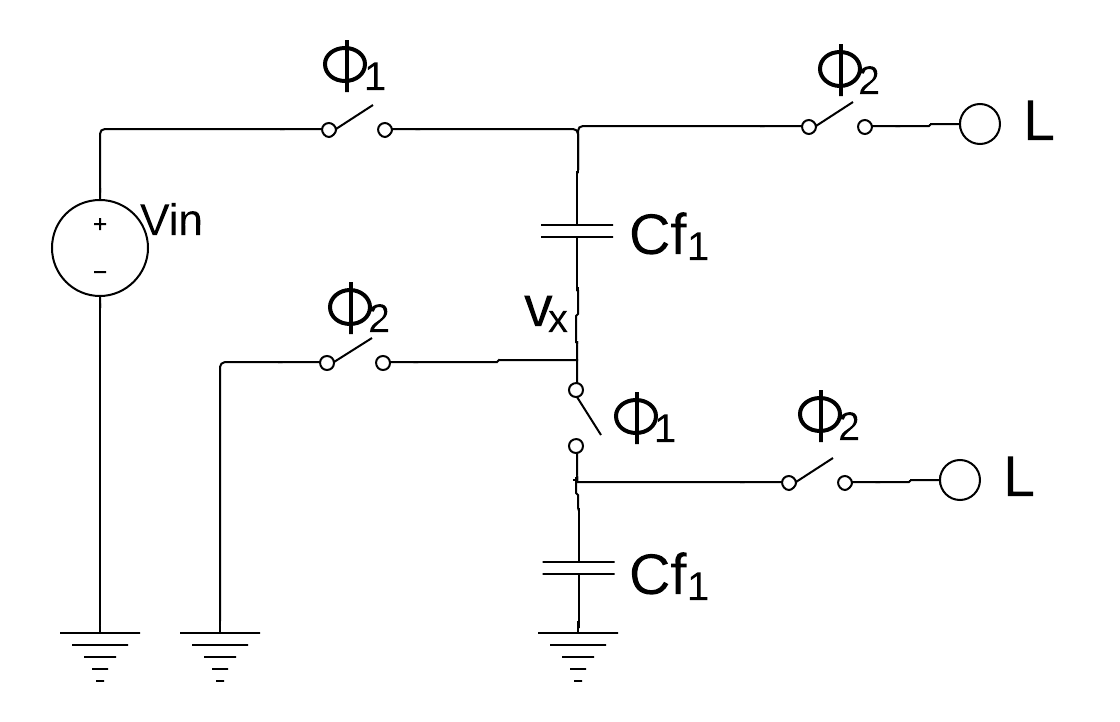
\includegraphics[width=0.4\textwidth]{SCTopology}
\caption{A $\frac{1}{2}$ stepdown SC topology}
\label{SCTopology}
\end{figure}

Let us consider the circuit with ideal components. $Cf$ denotes some capacitance such that $Cf_1 = Cf_2$. switches are controlled by mutually exclusive clocks, $\phi_1$ and $\phi_2$. These clocks are non-overlapping.\\
The circuit has two phases of operation. In phase 1, the charging phase, $\phi_1$ switches are closed and $\phi_2$ switches are open. $Cf_1$ and $Cf_2$ are in series. Since the capacitors are the same size, $V_x$ is $\frac{1}{2}$ of $V_in$.\\
In phase 2, the discharging phase, $\phi_2$ switches are closed and $\phi_1$ switches are open. Now $Cf_1$ and $Cf_2$ are in parallel. Since they are matched in size, $V_x$ remains at $\frac{1}{2}$ and is seen at terminal $L$ across both capacitors.\\

\subsection{Inductor-capacitor stepdown converter operating principle}

The second popular converter is the inductor-capacitor stepdown (buck) converter. A simplified canoical topology is shown in Figure~\ref{BKTopology}.\\
\begin{figure}[here]
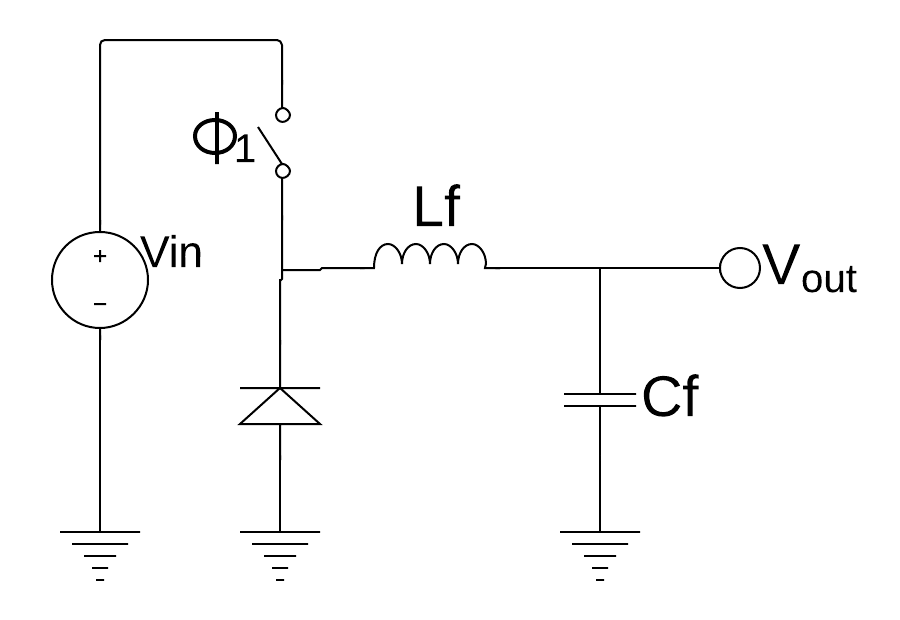
\includegraphics[width=0.4\textwidth]{BKTopology}
\caption{An inductor capacitor buck topology}
\label{BKTopology}
\end{figure}

%For Buck description use chapter 4 of Kurson
The voltage conversion principle is understood by considering the inductor and capacitor as a high pass filter. $\phi_1$ is a clock used to generate a square wave voltage of amplitude $V_{in}$. If this square wave is at a frequency sufficiently higher than the 3db cutoff frequency of the filter, only the DC component of the square wave is observed at $L$. Because of this, buck converters may change their voltage stepdown ratio during operation, by modulating $\phi_1$. For a properly designed converter, $V_L$ is defined by the duty cycle "$D$"~\cite{Kurson2006} of $\phi_1$ where: $V_{out} = V_{in} \times D$. In other words, if the square wave entering $L_f$ is high for $\frac{2}{3}$ of its period, $V_{out} = \frac{2}{3}\times V_{in}$ and $D = \frac{2}{3}$.\\ 

\subsection{SC stepdown converter critical parameters}
%Note the \textbf{introduction of $\phi_{\frac{2}{3}}$} This is introduced so when $Cf_2$ has discharged to the load, $Cf_1$ may be connected to restore the supply voltage seen at node $L$. \textbf{we do this because the parasitic resistance of $Cf_1$ and $Cf_2$ is larger in series, maintaining Vout for longer (also fucks with your load impedance, why do it??!!)}\textbf{WE SEE THAT IT IS CRITICAL TO HAVE HIGH FREQUENCY IN ORDER TO MAINTAIN SUPPLY VOLTAGE}
The energy that a SC converter can transfer per charge cycle is $E_{Isc} = CV^2$. We could therefore express $W = E_{Isc}\times F_\phi$.\\
$V$ For a design with a given $V_in$ and ideal components, the designer has two degrees of freedom to power a load, $C$ and $F_\phi$.\\  
We re-draw Figure~\ref{SCTopology} with non-ideal components in Figure~\ref{NonIdealSCTopology}.\\

By observation of Figure~\ref{NonIdealSCTopology} we see that $F_\phi$ and $C$ are critical parameters that must be optimised for minimum losses.\\
Losses associated with switches are switching loss during the non-overlapping period of $\phi$, and conduction loss due to the equivilent series resistance (ESR) of switches.\\
Conduction loss reduces the supply voltage seen at the capacitors by a factor $\delta V_a$. Conduction loss is therefore sensitive to the stepdown ratio. Increasing the stepdown ratio increases the number of series switches between all capacitors during the charging phase. For example a ratio of $\frac{1}{3}$ has 2 series switches, one of $\frac{1}{4}$ has 3 series switches and so on.\\
Losses associated with capacitors are parasitic capacitance losses. A parasitic capacitance known as bottom plate capacitance exists between one plate of each capacitor and ground. The voltage of these parasitic capacitor is a virtual ground and reduces the supply voltage seen at the capacitors by $\delta V_b$. Their charge can leak to true ground but cannot reach a load. As they are smaller than useful capacitance, they are significantly charged and discharged on each cycle of the converter. Loss is therefore expressed as $W = E_{Pc} \times F_\phi$ where $E_{Pc} = 1.5\alpha CV^2$. Literature reports bottom plate capacitance to be up to 5\% of $C_{tot}$~\cite{Ramadass2007}\\
%Move load regulation to different sub section SC converters by topology have difficulty 
In SC converters then, careful design considering voltage specification and technology parameters 

\subsection{Inductor-capacitor converter critical parameters}

How it works, critical parameters

\subsection{Converter load regulation concept}
Load regulation is matching output impedance "$Z_O$" of a power converter to a current load. Because $I= \frac{V}{Z_O}$ and maintaining $V$ for a processor is critical, converter output impedance must track quickly with the load condition to keep $V$ constant. The responsibility of tracking load and adjusting $Z_O$ belongs to control circuits. Block Diagrams are shown in figure~\ref{ControlCKBlockDiags}\\
Inductor-capacitor converters can reduce $Z_O$ by increasing conductance. This is done by increasing "$D$" in eqn\textbf{REF EQN}. Because the asymtote is impedance of the filter at $F_S$, $Z_O$ may also be increased by reducing $F_S$.~\cite{Alghamdi2012}.\\ %may want to change ref...
SC converters power loads capacitively. Because the capacitors supply a DC load in parallel, $Z_O$ cannot be lowered below $Z_C$ + $Z_{Sw}$ at the nominal $F_{Sw}$. Modulating $F_{Sw}$ can increase impedance in practice, because the capacitors can be purposely under-charged~\cite{Seeman2008}.\\
%Talk about tradeoffs? No I think put that in problems  

\section{Design of Integrated DC DC Converters}

Practical integrated converters are emerging and designed with different goals. A taxonomy of reviewed literature identifies two groupings:\\
\textbf{1: Power system replacement converters}. The goal is to remove external VRMs with an equaly performing integrated subsystem\\
\textbf{2: LDO replacement converters}. The goal is an incremental improvement of the Low-dropout (LDO) regulators that have long been integrated on chip~\ref{MaximLDO}.\\
These differing goals result in different design tradeoffs. We focus on group 1 because of an efficiency reason. To explain, consider the operating principle of an LDO. A transistor gate is biased in its linear conduction region and a fixed voltage is dropped from source to drain to give desired $V_{Out}$. Recall power transfer efficiency, $\eta = \frac{R_{Load}}{R_{Load} + R_{Source}}$. For an LDO, \textbf{(MAX)}[$\eta$] = 0.5. Using a comparable integrated converter to optimize power pins is intractable because around half the power budget is wasted as heat, clearly a sub-optimal design. As such, literature aiming at group 1 best aligns with our interest in pin count optimisation.\\  

\subsection{Motivation}
Switching converters such as the SC and buck can offer far higher efficient energy transfer than linear types. Theoretical efficiencies have been modeled at 96\%~\cite{Rodriguez2014} using state of the art devices. Integrated buck and SC implementations have been reported with 84\%~\cite{Cheng2013} and 93\%~\cite{Damak2013} efficiency respectively. Provided these power converters can drive the desired load of a processor, they could be used to obtain an optimum IO to power pin ratio for a processor. This would be done by increasing the input voltage to on die converters to reduce the number of supply pins until a desired number is reached.  

\subsection{Design challenges}
An Integrated DC DC converter is optimized through design tradeoffs that consider component non-idealities. Given that CPU designs have differing power envelopes and CMOS processes have unique electrical properties, researchers have explored the design space at multiple entry vectors.\\  

%\textbf{Definition of the system problem lives in}\\
%History of research\\
%System type 1(Switched capacitor AND HISTORY)\\
\indent \textbf{SC converters} The entry vector is an argument that A: Capacitance is easy to implement because MOSFET gate capacitance is a basic building block of CMOS. No corresponding basic block exists for inductance. B: Inductors have a necessarily large parasitic impedance because they are made from coiled resistive wire. Capacitors have a lower minimum impedance which shrinks as the plate size or capacitance grows.\\
However, as we have seen this type of converter has less flexible output impedance as compared with buck converters. Also SC converters do not have a voltage regulating filter which is built-in to bucks. This makes their output voltage vunerable to switching noise.\\
Therefore the design challenges emphasised in SC converters are: maximising effective capacitance, controlling output impedance and regulating output voltage.\\ 
%\textbf{Problems of bottom plate parasitic cap}. Bottom plate parasitic capacitance limits the attractiveness of SC designs. \\
%Problems of switching noise. These designs are noisier than Bucks, which have a filter by design\\
\indent \textbf{buck converters} The entry vector is an argument that C: Inductors can be implemented in standard CMOS. D: Inductor based buck has been a preferred design for (>100mW) applications over the past several decades ~\cite{Sanders2010}, why change now?
%System type 2(Integrated buck AND HISTORY Kurson book)\\
%Want to show how General CMOS components are made for this role and why they didn't work.\\

%MOVE THIS DOWN INTO THE NEXT SECTION
%In the case of both SC and buck, researchers faced setbacks from their initial vectors. We summarize these setbacks with reference to arguments \textbf{A},\textbf{B},\textbf{C} and \textbf{D}
%\begin{itemize}
%\item \textbf{A} CMOS MOSFET gate capacitance has large leakage and low energy density \textbf{CITE}
%\item \textbf{B} Parallel advances in device physics were applied to inductors, greatly improving inductance to impedance ratio \textbf{CITE}
%\item \textbf{C} CMOS implementations of inductors have low energy per area so were prohibitively area expensive \textbf{CITE}
%\item \textbf{D} Circuit design techniques alone cannot compensate for the quality of components realisable in standard CMOS \textbf{CITE} 
%\end{itemize}
%END MOVE DOWN

\subsection{Performance drawbacks of Baseline DC DC Converters}
An example of a CMOS integrated SC converter \cite{Viraj2007} and CMOS integrated buck converter \cite{Alimadadi2008} are taken as examples. These designs highlight the performance drawbacks of baseline CMOS for integrated converters and explain the present concentration of research interest in this field. These setbacks from the initial entry vectors of the SC and buck camps also explain the design approaches taken in more recent work.\\ 
\textbf{Taxonomy of problem (deeper drill and more specifics of the problem)}\\
what is wrong with the switches?\\ %loss of sqrt(fs) A 10-MHz Green Mode Automatic... Cite THIS paper.
what is wrong with the control? \\
What is wrong with the capacitors?\\
%.~\cite{Pique2012} evaluate the state of the art and plot an frontier of capacitor area to converter efficiency for Integrated converters. In general they find as capacitor area exponentially increases power density follows with only a linear cost in peak efficiency. However, efficiency exponentially decreases with power density in the non-ideal case. \\
What is wrong with the inductors?\\

\subsection{Solutions}
An evaluation of recent literature finds several novel approaches to the problems described previously. These are summarized below\\


\textbf{System: well defined, class of problems: well defined, now we will see "fixed" systems}\\
\begin{itemize}
\item{Switches fixes paper list and description DONT USE EXOTIC TECH! THESE WERE NEVER USED ON INTEGRATED DESIGNS!!!}
\item{Control fixes paper list and description NOTE THAT THIS PROBLEM IS WELL UNDER CONTROL, CONCLUDE FROM THIS SECTION}
\item{Capacitor fixes paper list and description NOTE THAT THIS PROBLEM CANNOT BE "SOLVED" FROM A SC TOPOLOGY POINT OF VIEW AND INDUCTORS ARE "BETTER" IN TERMS OF ENERGY DENSITY AND LINE REGULATION}
\item{Inductor fixes paper list and description. NOTE THAT THIS IS "SOLVED" BUT FOR SEMI-INTEGRATED OR WHATEVER}
\item{SC Ripple Fixes} % Fully Integrated Capacitive DC-DC Converter wit all digital Ripple Mitigation technique
\end{itemize}

\section{Saving pins with DC DC converters}

\textbf{Solutions \& Stakeholders, why is there still work to be done?}\\
Need to define the problem of Signal to power pin ratio. We cannot optimize this today with DC DC converters, because the \@ CMOS voltage stepdown means we need to have a lot of CORE power pins.\\
Our "stakeholder" is high voltage stepdown. If we do it we could reduce \textbf{DEFINE}"CORE POWER PINS" to an amount desirable for \textbf{DEFINE} signal integrity\\

\subsection{The IO limit with integrated DC DC converters}

\textbf{Defines stakeholder specific problem}\\
Think about this, it has to be differentiated from the section above

\subsection{Solutions}

Here we have to talk about:\\
3 the micro transformer solution to this problem (it could be made promising) \\
2 the MIT solution to this problem (it does not look promising)\\
1 the disruptive technology of Si on Insulator, and how it could be paired with interposers\\
In the mobile segment Silicon interposers can be used to solve the IO problem as seen in [Ultra-high I/O Density Glass/Silicon Interposer for high Band-witdh Smart Mobile Application].\\
This interposer allows signal integrity to be maintained at low voltage from the interposer to memory. a High voltage from the substrate and DC DC converter integrated to the interposer allows power density to be met with fewer pins on the package. In this scenario, the package can be made smaller to allow denser integration, or the io bandwidth  can be bound to signal integrity requirements...\\


\textbf{SHOULD HAVE SOME SIMULATION TO CHECK INSIGHT ON 1, 2 and 3}\\

\subsection{Conclusions}

Basically conclude that given the solutions simulation we could reach a situation where IO pressure is lifted from core power perspective, but that isn't so great tbh. 
  


{\footnotesize \bibliographystyle{acm}
\bibliography{sample.bib}}


\theendnotes

\end{document}







